\chapter{Background \& Objectives}
\section{The scenario}
The project is to create a system to produce real time holograms from a camera feed, using the Pepper’s ghost pyramid technique. The system is intended for use at the Aberystwyth Science Week next year, however, there was the potential to display a prototype at the 2017 event held in mid-March. The project is intended to show case a technique, originally used in stage and theatre productions, and give insight into how it can be adapted, with the aid of computer science, to make an impactful visual display.

The system will take real-time data captured from one from a staging area. The staging area will consist of a black background and appropriate lighting to illuminate the subject. The video feed will then be processed and displayed on a large monitor to work with a ghost pyramid of appropriate size.

To make the final demonstration more interactive, the display will have an accompanying system that allows users to play a charades style game. This would display a topic for the user to act out in the staging area and then allow those viewing the hologram to guess the activity being performed. This would require a system capable of taking multiple different string in puts (guesses) from users simultaneously, and feeding back to all users if a guess is correct. 

\section{Motivation and Justification}
This project is appealing due to the uniqueness of the technology being used to produce it. Whilst the charades game can be considered as a generic system, the creation of real-time holograms is not heavily developed. Many examples of video footage that can be used with the Pepper's Ghost Pyramid are readily available online, however there are far fewer implementation that do real time manipulation for this purpose.

Further to the project being interesting, it is designed with outreach events in mind. Already having an intended purpose means that it can be used as a helpful teaching tool for children to learn how basic physics and computer science can be used to create an interesting and engaging visual display. In addition, the charades game and real-time hologram system will help to further engage the audience with technique and visualise an impactful application of the technique. 

\section{Background}
\subsection{Pepper's Ghost Pyramid}
What was your background preparation for the project? What similar systems did you assess? What was your motivation and interest in this project?

The Pepper's Ghost technique was originally used for stage and theatre productions in the Victorian era to display holographic illusions to the audience. The technique, discovered by Dr. Henry Pepper, was first used in theatre in the 1860s\cite{pepper_ghost_comsol} and was used primarily to create a ghost-like illusion.

\begin{figure}[h!]
	\centering{
		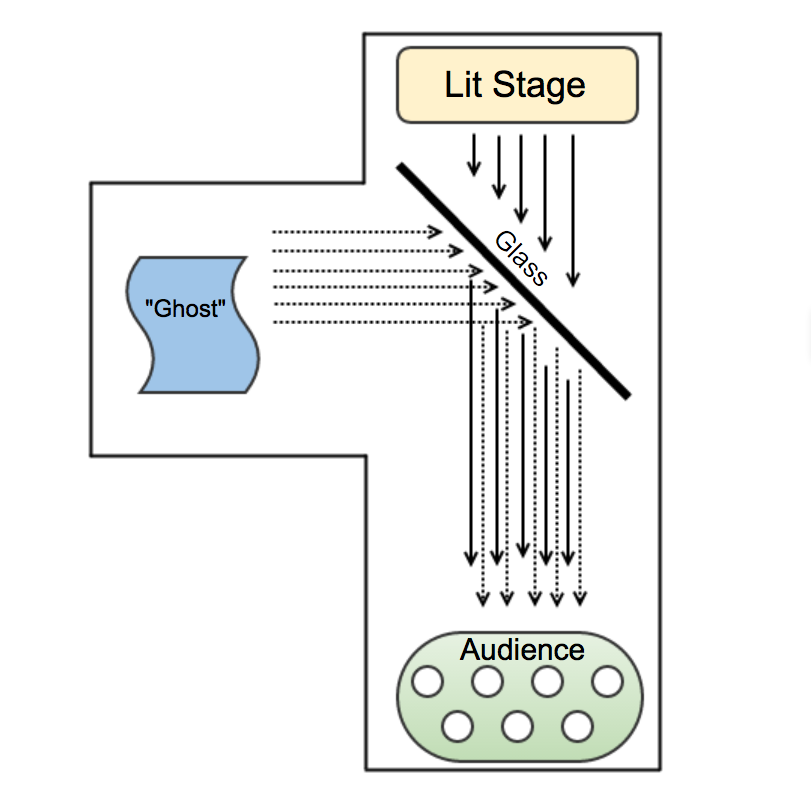
\includegraphics[scale=0.3]{Chapter1/basic_ghost.png}
		\caption{A basic diagram to display the Pepper's Ghost technique's use in theatre. The diagram dispicts how the audience are able to view the illusion where the solid lines represent light  from the lit stage and dashed lines as light rays from the "Ghost". The image has been taken from reference \cite{pepper_ghost_comsol}.}
		\label{fig:basic_ghost}
	}
\end{figure}

Figure \ref{fig:basic_ghost} shows a basic example of how the technique produces holographic illusions. The lit stage that is parallel to the viewers line of sight will have actors and scenery as per a normal stage production. The "Ghost" is located off stage and is not visible by the audience. When illuminated, the ghost is displayed to the audience as the light ray travel radially from the "Ghost" and those that reach the glass will be refracted. The glass is positioned at 45\textdegree{} from both the audience and the "Ghost" to allow account for the 90\textdegree{} offset between the two.

Since the 1860s, this technique has been used in different settings and has proven popular in museums and exhibitions such as \textit{An Audience with Sir Alex Ferguson} at the Manchester United Football Club museum \cite{alex_ferguson} and \textit{Shane Warne - 'Cricket Found Me'} at the national sports museum in Melbourne \cite{shane_warne}. In more recent years, there has been a resurgence in the use of the technique on a smaller scale, and this has continued to thrive in popularity due to the ease of access to materials and the availability of information regarding the technique.

Whilst the technique still uses Henry Pepper's original concept, it has been modified to display the hologram from multiple angles using a pyramid - rather than a single glass plane. This structure is commonly referred to as the Pepper's Ghost pyramid.
\begin{figure}[h!]
	\centering{
		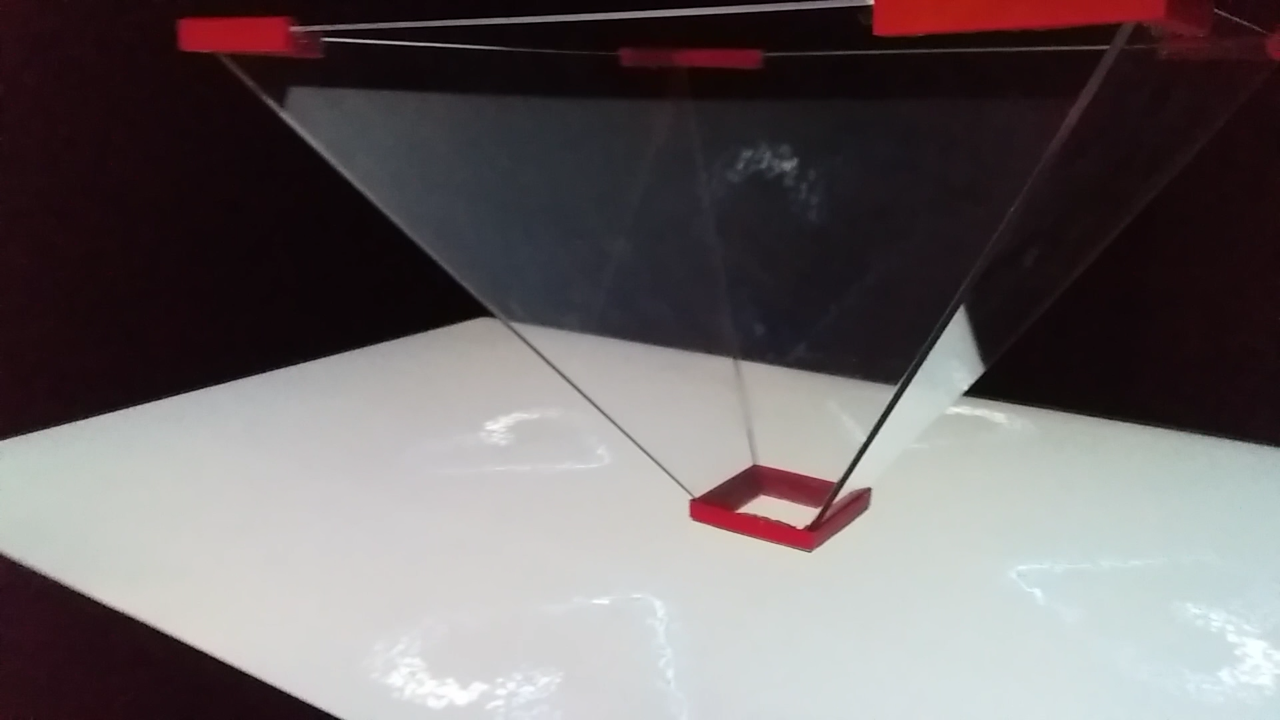
\includegraphics[width=\linewidth]{Chapter1/ghost_pyramid.png}
		\caption{An image of modern day Pepper's Ghost Pyramid made from clear acrylic. This was constructed and is own by Aberystwyth University Computer Science Dept. In the Figure, the pyramid is located on a large monitor that is being used to display the hologram input images.}
		\label{fig:ghost_pramid}
	}
\end{figure}

Figure \ref{fig:ghost_pramid} shows an example of a Pepper's Ghost pyramid. The pyramid is square based, made from a transparent material (such as perspex, clear acrylic or glass) and is open at both the top and bottom. The technique for displaying holograms differs with the "Ghost" now being an image or video displayed on a screen. Furthermore, to create an illusion from all sides of the pyramid, four images are required (one for each side of the pyramid). This  means that the 2D projection of the image can be seen from any side of the pyramid. This Pyramid structure is what will be used for the hologram creation part of this project.

\textit{Whilst the pyramid implementation is an improvement on Pepper's original design it still suffers from the some of the same limitations of the original. The original design is reliant on the viewer looking directly at the transparent plane which makes it both vertically and horizontally intolerant for the viewer. The pyramid implementation means that the hologram is visible from four perspectives (in front, behind, left and right). Whilst this is an improvement, the hologram is not easily viewed from the edges of the pyramid and does not affect the vertical intolerance as viewing from above is not possible. Some concepts for a spherical design (instead of a pyramid) are proposed to resolve the horizontal intolerance completely.}

\section{Analysis}
\textit{Taking into account the problem and what you learned from the background work, what was your analysis of the problem? How did your analysis help to decompose the problem into the main tasks that you would undertake? Were there alternative approaches? Why did you choose one approach compared to the alternatives? \\
There should be a clear statement of the objectives of the work, which you will evaluate at the end of the work. \\
In most cases, the agreed objectives or requirements will be the result of a compromise between what would ideally have been produced and what was determined to be possible in the time available. A discussion of the process of arriving at the final list is usually appropriate.\\
As mentioned in the lectures, think about possible security issues for the project topic. Whilst these might not be relevant for all projects, do consider if there are relevant for your project. Where there are relevant security issues, discuss how they will this affect the work that you are doing. Carry forward this discussion into relevant areas for design, implementation and testing.}


Whilst there have been numerous examples of application using the Pepper's Ghost Pyramid as a computer visualisation technique, none where found that detailed using this as part of a real-time system. Furthermore, whilst many have used the technique in an educational setting, it is more often that the content of the hologram is used as an educational aid, rather than focusing on the technique itself. Due to its simplicity, the Pepper's Ghost technique is ideal to help younger children understand light and refraction.  

\subsection{Objectives}
Initially the project scope covered the creation of a system to produce real-time holograms using a video feed. Considering the time-line of the project and the work involved, the addition of an accompanying system for the Charades game was later added to the Objectives.
The objectives that were agreed upon are as follows:
\begin{itemize}
	\item To produce a system that can be used for outreach events to show case the creation of holograms using the Pepper's Ghost Pyramid.
	
	\item The system should use real-time video to capture a member of the audience and then project these images as holograms using the Pepper's Ghost Technique.
	
	\item An accompanying system should be produced to allow for a charades style game to be played using the primary system as the display for the actor.
	
	\item Given the target audience, the system should be interactive and engaging whilst also enabling the viewers to learn about what the technique is and how it works.
	
	\item The system should be easy to use and require little explanation.
	
	\item As it is design for use at outreach events, the system should be robust and the thoroughly tested.
	
	\item The system should be easy to run from the perspective of the client. Initial set up should ideally be straight forward and self explanatory.
\end{itemize}


\subsection{Problem decomposition}
Following the agreement of the project objectives, it was possible to begin to decompose the requirements of the project into smaller sections. As the project is comprised of two systems (The real-time Pepper's ghost creation system and the charades game), this seemed a natural divide for the project at the highest abstraction layer.

\subsubsection{Real-time Pepper's ghost}
Background reading about the Ghost Pepper's technique helps to unveil its simplicity and ease of implementation. As such, it was decided that a prototype of the hologram system would be created for the 2017 Aberystwyth University Science Week event. The main tasks to produce this system involve:
\begin{itemize}
	\item Analysis and Design of the display and staging area. Both the area in which the holograms are viewed in, as well as the area were a viewer would be filmed, needed to be considered to assess the feasibility of the system.
	\item Obtaining a live camera feed from a webcam in a format that can be manipulated.
	\item Correctly orientate and position multiple copies of the camera feeds in a single display window.
	\item Ensure the video feed is of the correct size and scale for the output device.
\end{itemize}

The main consideration throughout the development process of the Pepper's ghost application is the efficiency of the video feed manipulation. To have an effective display the video should be running at no less than 30 frames per second with an ideal target so closer to 60 frames a second depending on the capture speed of the camera.
 
\subsubsection{Charades game}
The charades game will form the more interactive side of the project. The concept is to have a single actor (member of the audience) outside the viewing area with a tablet or phone. They will select a phrase from a choice of phrases and then act out that phrase. The acting will be captured by the webcam from Pepper's ghost system and displayed as a hologram in the viewing area. Whilst the phrase is being acted, the viewers (who will also have a tablet or phone) will be given information about the phrase (such as the number of words and the genre of the phrase) and will attempt to guess what is being acted. Once the phrase has been successfully acted, the actor will be prompted to select a new phrase and the viewers will be given points. After three phrases, the winner will be the viewer with the most points. The main tasks of the charades game will be:
\begin{itemize}
	\item Creating a user interface for both the actor and viewer.
	\item Allowing the actor to select a phrase and, if the phrase is comprised of multiple words, a current word to act.
	\item Allowing the viewer to attempt to guess the current word or phrase
	\item Inform both users when the word or phrase has been correctly guessed.
	\item Prompt the actor for a new word or phrase for them to act.
	\item Establish and implement how and when the game ends.
	\item Inform users of the winner.	
	\item Create a session system to only allow those who have logged on to the website with the correct details to access the information. 
\end{itemize}

Despite the system only being designed for localised use at events, a web hosted implementation would be best to allow user to access the system from their own mobile devices (or those supplied by the event organiser). However, this does raise certain additional security issues that should be taken into consideration which include ensuring that only those at the event can access the system. To do this, a session concept is listed as part of the main tasks to be completed. This will ensure that only those with the session key are able to access the system. The system should also provide the ability to change the session key easily when required.

\subsection{Alternative implementations}
The charades system has been implementation as a website however initially the design was for an android application. An android application boasts the increase security as devices could potentially connect via Bluetooth. Furthermore, it would stop users from attempting to change the information in the URL for each page and therefore reduce the number of check required to ensure that the system data had not been tainted.
Despite this, a web application done correctly is more accessible to users as it is platform independent. Meaning that the university would not have to invest in android specific devices in order to access the system. In addition, it would be more likely that users can access the system from their own devices meaning more users can play the game at the same time.

\section{Process}
The development of this project followed the Feature Driven Development (FDD) plan driven methodology. FDD is normally considered for larger projects as it provides a framework for distributed development. By dividing developers into smaller teams, FDD allows those teams to tackle features one at a time in parallel. Furthermore, the up front planning stage is generally indicative of projects that are more stable as, whilst it can be adapted throughout the process, the overall model is normally only added to, and the core architecture remains static.

The steps required to complete this project are well defined and therefore would be well suited to having up front design. Furthermore, FDD encourages continuous integration (CI) which offers  a good way to produce a functional prototype at various stages of the project. CI will be a significant aid for the mid project review and potentially testing a prototype with users at the 2017 Aberystwyth University science week event.

\subsection{Single Person FDD adaptation}
To successfully use FDD for this project, several adaptations to the normal processes of the methodology will need to be made. The most notable is the abolition of the developer teams in favour of a single developer. This requires the developer to assume multiple roles throughout the development process and at each different stage.

\subsubsection{Develop an Overall Model}
Initially, a Domain Expert (Customer) is required to aide in the development of the overall model and feature creation. In this context, the project supervisor can fulfil this role and the developer shall act as both the Chief Programmer and Chief Architect. For this project, the Domain specific language is shared by both the Domain Expert and the developer.

\subsubsection{Build a Feature list}
The feature list produced will form the requirements list for the project. This will be generated from discussion between the developer and the Domain Expert and then when complete will be verified by both parties.

\subsubsection{Plan by Feature}
Steps such as establishing developer teams and scheduling developer teams time throughout the project no longer exist. In their place, the features can be given priorities that will aide in time scheduling and development order. Once the order is created, the features can be assigned to separate iterations.

\subsubsection{Design by Feature}
Once a feature is selected, that feature will be exhaustively designed taking into consideration the functions required to fulfil the feature. The project uses GitHub for version control and an issue will be created which corresponds to a feature. The first action in an issue will be to complete a design of the feature and update the overall design as required.

\subsubsection{Implement by Feature}
Features will be implemented in the same GitHub issue as the design work. The project is being developed using TDD and therefore, the test suite will be updated before any code is implemented. Once the tests are created, an implementation is then added and this must pass the tests to be acceptable. Whilst the tests can be run locally, there will also be a Jenkins service for continuous integration to run the full test suite before it can be merged with the master branch.  

To allow for a code review/walk through, completed features are to be left as open pull requests for a day before reviewing the code to ensure good quality code is created for each feature.